% !TEX TS-program = pdflatexmk
\documentclass[12pt]{article}

\usepackage{pgf,tikz}
\usetikzlibrary{arrows}

% Layout.
\usepackage[top=.75in, bottom=0.75in, left=.75in, right=.75in, headheight=1in, headsep=6pt]{geometry}
\usepackage{subfig}
% Fonts.
\usepackage{mathptmx}
\usepackage[scaled=0.86]{helvet}
\renewcommand{\emph}[1]{\textsf{\textbf{#1}}}

% Misc packages.
\usepackage{amsmath,amssymb,latexsym}
\usepackage{graphicx,tikz}
\usepackage{array}
\usepackage{xcolor}
\usepackage{multicol}
\usepackage{tabularx,colortbl}
\usepackage{amsthm}
\usepackage{enumitem}
%to make tikz pics work
\usepackage{tikz,pgfplots}
\usepackage{float}
\newcommand\solution{\localhead{Solution:}}

\usepackage[colorlinks=true]{hyperref}

% Paragraph spacing
\parindent 0pt
\parskip 6pt plus 1pt
\def\tableindent{\hskip 0.5 in}
\def\ts{\hskip 1.5 em}

\usepackage{fancyhdr}
\pagestyle{fancy} 
\lhead{\large\sf\textbf{MATH 663 }}
\rhead{\large\sf\textbf{Fall 2023}}
\chead{\large\sf\textbf{HW 1}}

\newcommand{\localhead}[1]{\par\smallskip\textbf{#1}\nobreak\\}%
\def\heading#1{\localhead{\large\emph{#1}}}
\def\subheading#1{\localhead{\emph{#1}}}

%% Special Math Symbol shortcuts
\newcommand{\bbN}{\mathbb{N}}
\newcommand{\rad}{\text{rad}}
\newcommand{\diam}{\text{diam}}
\newcommand{\circumference}{\text{circ}}

%\newenvironment{clist}%
%{\bgroup\parskip 0pt\begin{list}{$\bullet$}{\partopsep 4pt\topsep 0pt\itemsep -2pt}}%
%{\end{list}\egroup}%

\usetikzlibrary{calc}
%\pgfplotsset{my style/.append style={axis x line=middle, axis y line=
%middle, xlabel={$x$}, ylabel={$y$}, axis equal }}


\begin{document}
\begin{enumerate}

	\item Determine the number of edges in a complete graph on $n$ vertices.
	\begin{proof} 
		Suppose $G$ is a complete graph on $n$ vertices. There exists $n \choose 2$ ways of pairing vertices. Since $G$ is a complete graph, each pair of vertices correspond to an edge. Hence there are $n \choose 2$, or $\frac{n(n - 1)}{2}$ edges. 
	\end{proof}
	\vspace{.5in}


	\item Let $d \in \bbN$ and $V=\{0,1\}^d.$ That is, $V$ is the set of all binary sequences of length $d.$ Define a graph on $V$ in which two sequences form an edge if and only if they differ in exactly one position. (This graph is called the \emph{d-dimensional cube}.) 
		\begin{enumerate}
			\item Draw and label the vertices of the 1-, 2-, and 3-dimensional cube.\\
				\solution

					\begin{figure}[H]
					    \centering
					    \subfloat[\centering $d = 1$]{{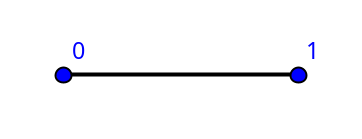
\includegraphics[width=4.5cm]{d1.png} }}
					    \qquad
					    \subfloat[\centering $d = 2$]{{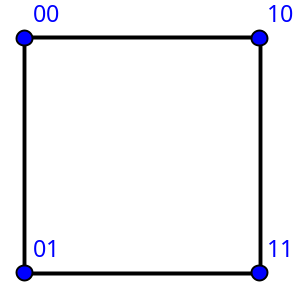
\includegraphics[width=3cm]{d2.png} }}\\
						\subfloat[\centering $d = 3$]{{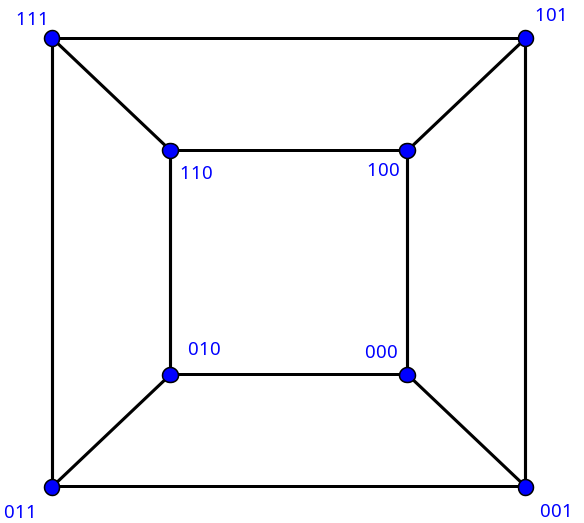
\includegraphics[width=7cm]{d3.png} }}
						\caption{d-dimensional cubes.}
					    \label{fig:-cubes}%
					\end{figure}




			\item Determine the average degree, number of edges, diameter, girth and circumference of the $n$-dimensional cube.
				\solution Let $n \in \bbN$ and $V=\{0,1\}^n.$ Suppose a graph $G$, on $V$ in which two sequences form an edge if and only if they differ in exactly one position. 
					\begin{proof}
					To determine $d(G)$ note that for a given, length $n$ binary sequence there are $n$ unique ways to differ exactly one position. Hence $G$ is $n$-regular and thus $d(G) = n$. 
					\end{proof}
					\vspace{.15in}

					\begin{proof}
						Clearly $|V| = 2^n$, and since $G$ is $n$-regular it follows $|E| = \frac{1}{2}2^nn = 2^{n - 1} n$.
					\end{proof}
					\vspace{.15in}

		
					\begin{proof}
					To find the $g(G)$ first note that if $n = 1$ then $g(G) = 0$ since there exists no cycle. Now note that for $n \geq 2$ there will exist vertices which correspond to the sequences $11\dots, 01\dots, 10\dots, 00\dots$ with trailing zeros after the first two indices. These vertices, by definition must form a 4-cycle. Hence $g(G) = 4$. 
					\end{proof}
					\vspace{.15in}


		\begin{proof} I assert $\diam(G) = n$. Let $x$ and $y$ be vertices in $G$ and suppose 
			$k$ is the number of differing positions between $x$ and $y$. We assert that $d(x, y) = k$. If $d(x, y) < k$ then there would be an edge incident to vertices that were more than one position apart. Since two vertices can differ in at most $n$ positions $\diam(G) = n$. 
			\end{proof}
	\vspace{.15in}


	
		\begin{proof}
		I assert that the $\circumference(G) = |V(G)| = 2^n$. We will proceed to show that the $n$-dimension cube has a Hamiltonian cycle, for all $n \geq 2$. The base case is trivial as the $2$-dimension cube is a four cycle.\\

		Let $G_0$ and $G_1$ be two disjoint but identical $n$-dimensional cubes. By the induction hypothesis $G_0$ and $G_1$ have 2 identical Hamiltonian cycles $H_0$ and $H_1$ respectively. We construct a new graph $G$ by, 
		\begin{align*}
			V(G) &= V(G_0) \cup V(G_1)\\
			E(G) &= E(G_0) \cup E(G_1) \cup \{ xy: x \in V(G_0), y\in V(G_1), x = y \}
		\end{align*}
		Now relabel each vertex from $G$ based on the following map $f: G \to G'$ where $G'$ is an $n + 1$ dimensional cube,
		\begin{equation*}
			f(x) = \begin{cases}
				x0 & x \in V(G_0)\\ 
				x1 & x \in V(G_1)
			\end{cases}
		\end{equation*}


		This map is clearly a bijection between vertex sets. Now consider some $xy \in E(G)$. We know that either $x, y \in V(G_0)$, $x, y \in V(G_1)$, or without loss of generality $x\in V(G_0)$ and $y \in V(G_1)$. For the former two, since $f$ appends the \emph{same} bit to \emph{both} vertices, $f(x)$ and $f(y)$ differ by only one position and therefore $f(x)f(y) \in G'$.

		For the latter case since $xy \in E(G)$ and $x\in V(G_0)$ and $y \in V(G_1)$ it follows by our definition of $E(G)$ that $x = y$ and therefore since $f$ appends a \emph{different} bit to \emph{identical} vertices $x$ and $y$ we know that $f(x)$ and $f(y)$ differ in the last position, so $f(x)f(y) \in G'$.\\


		Thus $G$ is an $n+1$ dimensional cube. Finally we construct a new Hamiltonian cycle by swapping a pair of edges. Note there exists some edge in $H_0$ incident to vertices $x10$ and $x00$, and similarly $H_1$ has an edge incident to vertices $x11$ and $x01$. Remove them, and replace them with the edge incident to $x10$ and $x10$ and the edge incident $x00$ and $x01$. These new edges must exists by construction of $G$ and connect to form a Hamiltonian cycle on $G$.
	\end{proof}

\end{enumerate}
\vspace{.5in}




\item  Let $G$ be a graph containing a cycle $C,$ and assume that $G$ contains a path of length at least $k$ between two vertices of $C$. Show that $G$ contains a cycle of length at least $\sqrt{k}$.
\begin{proof} Let $G$ be a graph containing a cycle $C$, let $x_0$ and $x_k$ be vertices of $C$ and suppose that $G$ contains a path $P$ of length at least $k$ between two vertices $x_0$ and $x_k$. 
Now consider a subset of vertices, $V(P) \cap V(C)$ and note that if $|V(P) \cap V(C)| \geq \sqrt{k}$ it follows that $C$ is a desired cycle of length at least $\sqrt{k}$.

	Otherwise suppose $|V(P)\cap V(C)| < \sqrt{k}$. Note that the vertices of $V(P) \cap V(C)$ partition the $k$ edges of $P$, via $|V(P) \cap V(C)| - 1$ subpaths. Therefore must exists a subpath $P_i$ with
	terminal vertices, $x_i$ and $x_{i + 1}$ in $C$ with length at least 
	\begin{equation*}
		\dfrac{k}{|V(P) \cap V(C)| - 1} \geq \dfrac{k}{\sqrt{k} - 1}> \sqrt{k}.
	\end{equation*}
	It is clear that the path between $x_i$ and $x_{i + 1}$ through $C$, and $P_i$ form a cycle with 
	length greater than $\sqrt{k}$.
\end{proof}
\vspace{.5in}







\item Proposition 1.3.2 states that Every graph $G$ containing a cycle satisfies, 
$$g(G) \leq 2\diam(G) + 1$$ Is this bound best possible? Prove your answer is correct.
\begin{proof} I assert that $2\diam(G) + 1$ is the best possible bound. Consider a cycle $C^{5}$, clearly $g(C^5)$ and $\diam(G) = 2$ so we conclude that,
	\begin{equation*}
		g(C^5) = 5 = 2(2) + 1 = 2(\diam(C^5)) + 1.
	\end{equation*} 
\end{proof}
\vspace{.5in}


\item Show that for every graph $G$, $\rad(G) \leq \diam(G) \leq 2\rad(G).$
\begin{proof} Let $P$ be some path from $x_0$ to $x_k$, such that $|P| = \diam(G) = k$. Let
	$x_c$ be a central vertex, $P_0$ to be a minimal path between $x_0$ and $x_c$ and,
	$P_k$ be the minima path between $x_c$ and $x_k$. It follows, since $x_c$ is central 
	that $|P_0|, |P_k| \leq \rad(G)$. Construct a walk $W = x_0P_0x_cP_kx_k$ and note that since $P$ is a shortest path we get, 
	\begin{equation*}
		\diam(G) = |P| \leq |W| = |P_0| + |P_k| \leq 2\rad(G).
	\end{equation*} 

	Note that $\rad(G) \leq \diam(G)$ is attained by definition, since
	\begin{equation*}
		\rad(G) = \min_{x \in V(G)} \quad \max_{y \in V(G)} d_G(x, y),
	\end{equation*}
	\begin{equation*}
		\diam(G) = \max_{x \in V(G)} \quad \max_{y \in V(G)} d_G(x, y). 
	\end{equation*}
\end{proof}

% rad(G) = the minimal maximal distance between any two vertices. The maximal distance between 
% the central vertex and any other vertex. 
\end{enumerate}

\end{document}


